\chapter{Discussion}
In the above chapters, we presented results about how gene regulatory networks
self-organize and the dynamics of which is governed by its topology. We explored
the cellular signal flow scheme by means of calculating the nodal distances in
the protein interaction network. Our results have several interesting implications
as to the general design principles of cellular interaction networks and
how we can utilize them to reverse-engineer those interaction networks.

\section{Cellular attractor}
In \ref{chap:network}, we learned that those strongly perturbed genes are
correlated with the cellular phenotype, while remaining sparsely connected in
the gene regulatory network. This result raises the question, what are the
functions of the other densely connected but moderately regulated genes? 
To answer this question, it is beneficial to consider the gene regulatory network
as a cellular attractor.

The origin of the cellular attractor probably stems from the idea of 
\emph{epigenetic landscape} by Conrad Waddington in the 1950s 
(\ref{fig:landscape}). It basically
states that different cell types can be visualized by valleys in a landscape,
and the cell differentiation process is essentially a marble rolling down to
different points of lowest local elevation. The formalization of the epigenetic landscape notion opens the door to the understanding of the key role played by stochastic fluctuation. 
It is however important to note that Waddington uses the term \emph{epigenetic} in a broader sense than in modern molecular biology where it refers to the apparently irreversible covalent DNA and chromatin modifications that influence expression of individual genes.

\begin{figure}[!ht]
\begin{center}
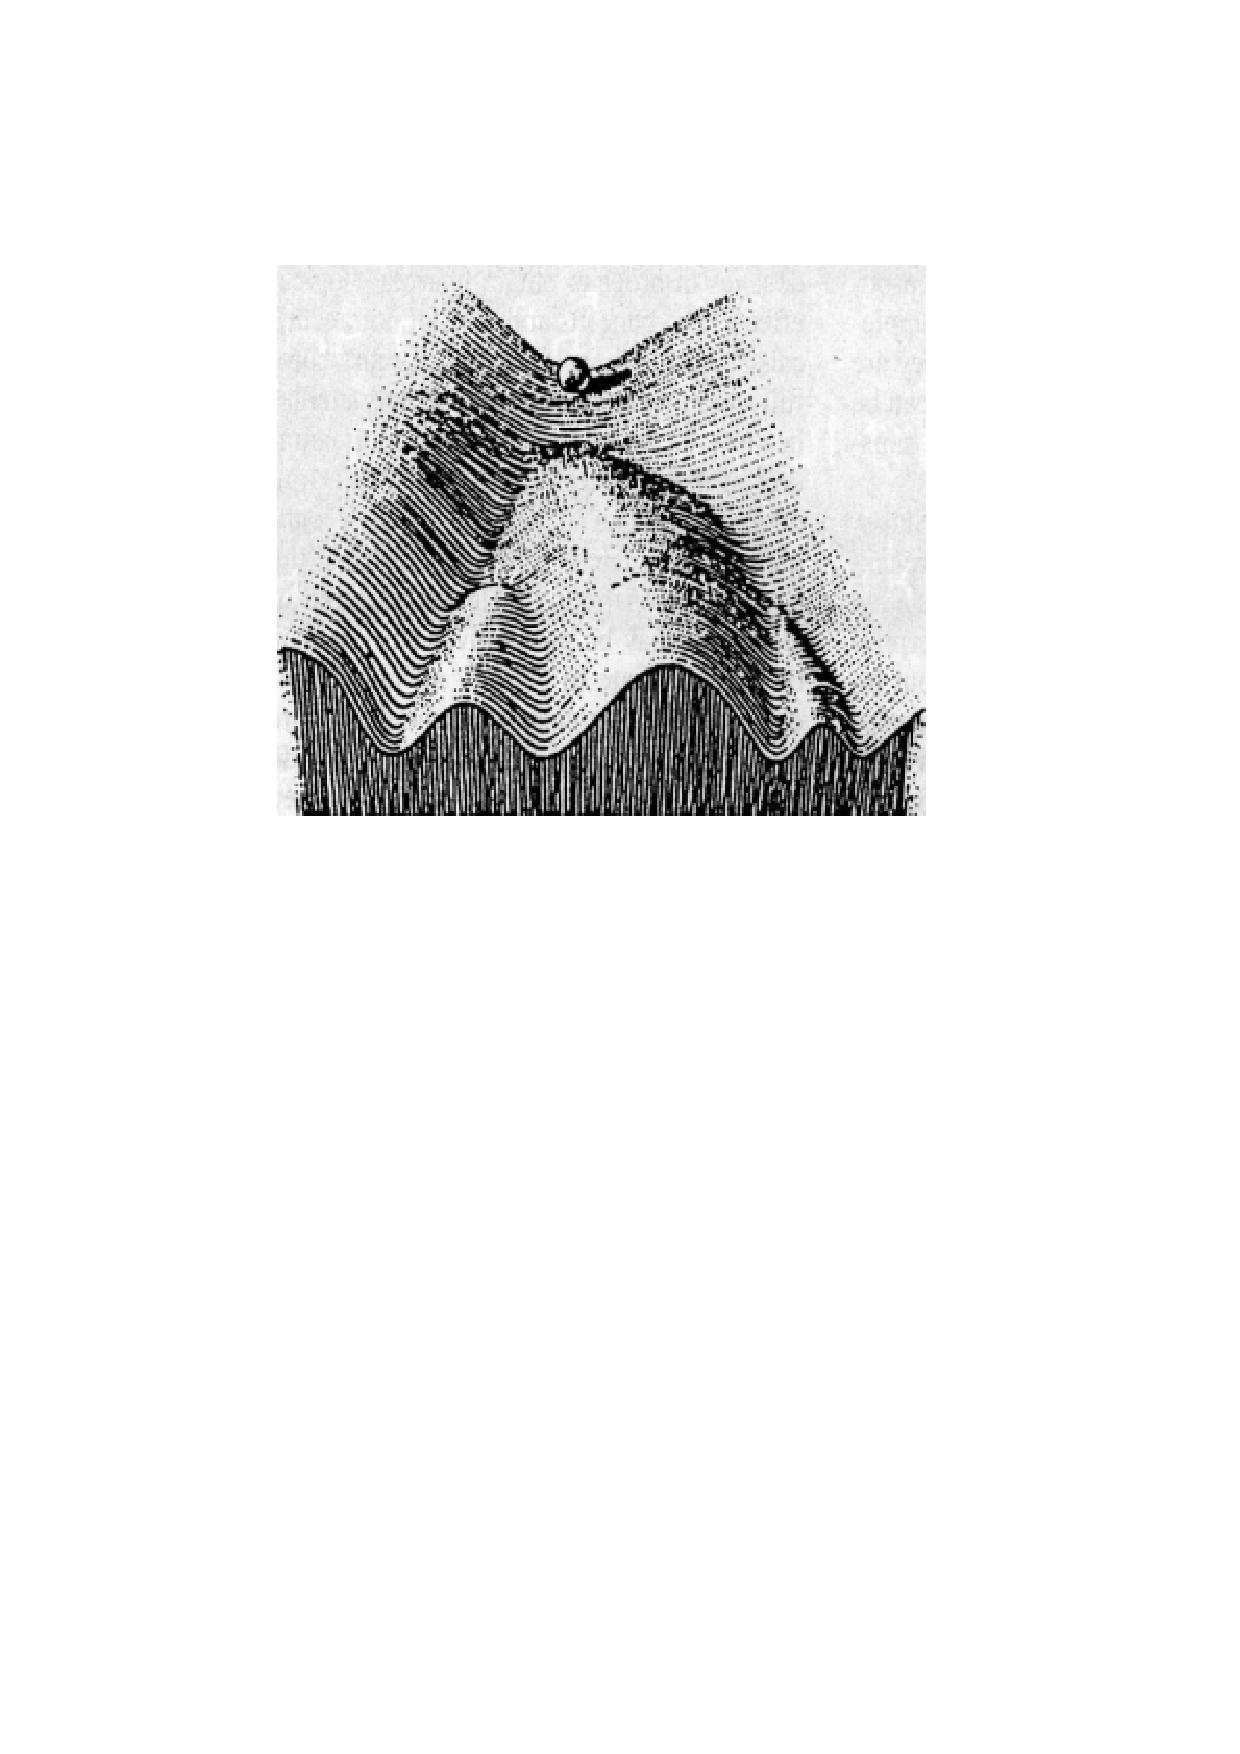
\includegraphics[width=0.8\textwidth]{landscape.pdf}
\end{center}
\caption[Waddington's epigenetic landscape]{
{\bf Waddington's epigenetic landscape.}
The marble represents a cell state. The overall slope represents the driving force of development. As the marble rolls downwards, the cell is forced to choose between discrete fates represented by the valleys.
}
\label{fig:landscape}
\end{figure}

Using a random Boolean network approach, \cite{Kauffman1969a} postulated that high-dimensional attractors of genomic networks represent cell types, thereby effectively
extending the notion of attractors from phenotypes to molecular interaction
networks.
In dynamical systems theory, the attractor landscape can also be naturally 
understood as steady states of the system, which is determined by the system 
parameters.
The relative size, shape, and distribution of the basins of
attraction in the $N$-dimensional hyperspace of gene configurations restrict the patterns with which the system will
transit from one attractor to another in time and space.

It was further suggested that the attractor can also be associated with distinct cell fates, or functional phenotypes, such as the proliferative, quiescent, migratory or differentiated state of all cell types, thus representing high-dimensional 
steady states of the gene regulatory network~\citep{Huang2006,Huang2005}.
Attractor states, that is, the \emph{low-energy} valleys in the landscape, indeed share fundamental properties with cell fates in that they are discretely distinct functional states, essentially mutually exclusive and can undergo a switch-like transition from one to another. The change of cell fate can then be viewed from a new
perspective as transition between
attractors. A non-specific external signal can also induce phenotypic changes by
simply destabilizing the network state 
away from the attractor, the network itself then selectively moves into another
accessible attractor.

Taking as an example the neutrophil differentiation through two different stimuli, dimethyl sulfoxide (DMSO) and all-trans-retinoic acid (atRA), \cite{Tsuchiya2010}
analyzed the gene expression dynamics in correlation space defined by Pearson correlation and mutual information. It was shown that the probability distributions of
correlation for both stimuli converge after 48 hours, defining the neutrophil attractor. They noticed that only genes with low or moderate expression changes, which are often considered noisy and insignificant, are essential components of the neutrophil attractor. This work highlights the function of moderately regulated genes as 
driving force of the phenotype, which only became comprehensible in the context
of cellular attractors.

As yet another example, \cite{Busch2013} applied a correlation trajectory analysis of the 
time-resolved transcriptome data in the moss leaflet apical stem cell development, 
and predicted the important role of 
moderately regulated transcription factors in triggering developmental 
decisions. The methodology successfully narrowed down a total of 1,058 TFs to 
5 candidates that are likely to be involved in the signaling leading to the establishment of pluripotency in apical stem cells. One of the predicted bHLH TFs PpRSL1 has previously been described as a positive regulator of caulonema and rhizoid development, 
its involvement in the establishment of \emph{P. patens} apical stem cells is also confirmed
in the loss-of-function mutants.

\section{Topology-constrained reverse-engineering of gene regulatory networks}
As stated in \ref{sec:strong_regulator_phenotype}, our finding that strongly perturbed 
genes are sparsely connected has important implications for the reverse-engineering
of gene regulatory networks. Although posed by many people and attempted by 
many theoretical framework, the inference of gene regulatory networks from 
high-throughput microarray data remains a big challenge. It was learned from
the initiative of Dialogue on Reverse Engineering Assessment and Methods (DREAM),
that no single inference method performs optimally across all data sets. 
It is only through the integration of predictions from multiple inference methods 
that one can achieve a highly robust and accurate prediction~\citep{Marbach2012}.

The reverse-engineering of gene regulatory networks finally boils down to 
estimating the model parameters from experimental data. The difficulty of
parameter estimation lies in the intrinsic high dimensionality of the search
(parameter) space. Therefore, one way to overcome this difficulty is to 
constrain the search space, in the way that one incorporates prior knowledge
about the model system. In our case, a potentially useful prior knowledge
about the gene regulatory network is the sparse connectivity of strongly 
responding genes.

There are at least two options to implement this topological constraint. 
First, one can take the topological prior knowledge as an additional
criterion in the optimization. Any of the parameter estimation problem
can be seen as an optimization problem, in that one defines a certain
objective function and iteratively tune the parameters to search for
the optima of this objective function. The objective function is usually the 
dissimilarity between the experimental data and the simulation with a certain
set of parameters (for example
relative standard error). The topological prior knowledge can be incorporated
into the parameter estimation by adding a penalization term to the
objective function.
One can for example
assign a high cost to the genes that have an undesired degree (\ref{fig:cost_function}), 
which is exactly derived 
from the observation that the response strength of a gene and its connectivity
are negatively related.

\begin{figure}[!ht]
\begin{center}
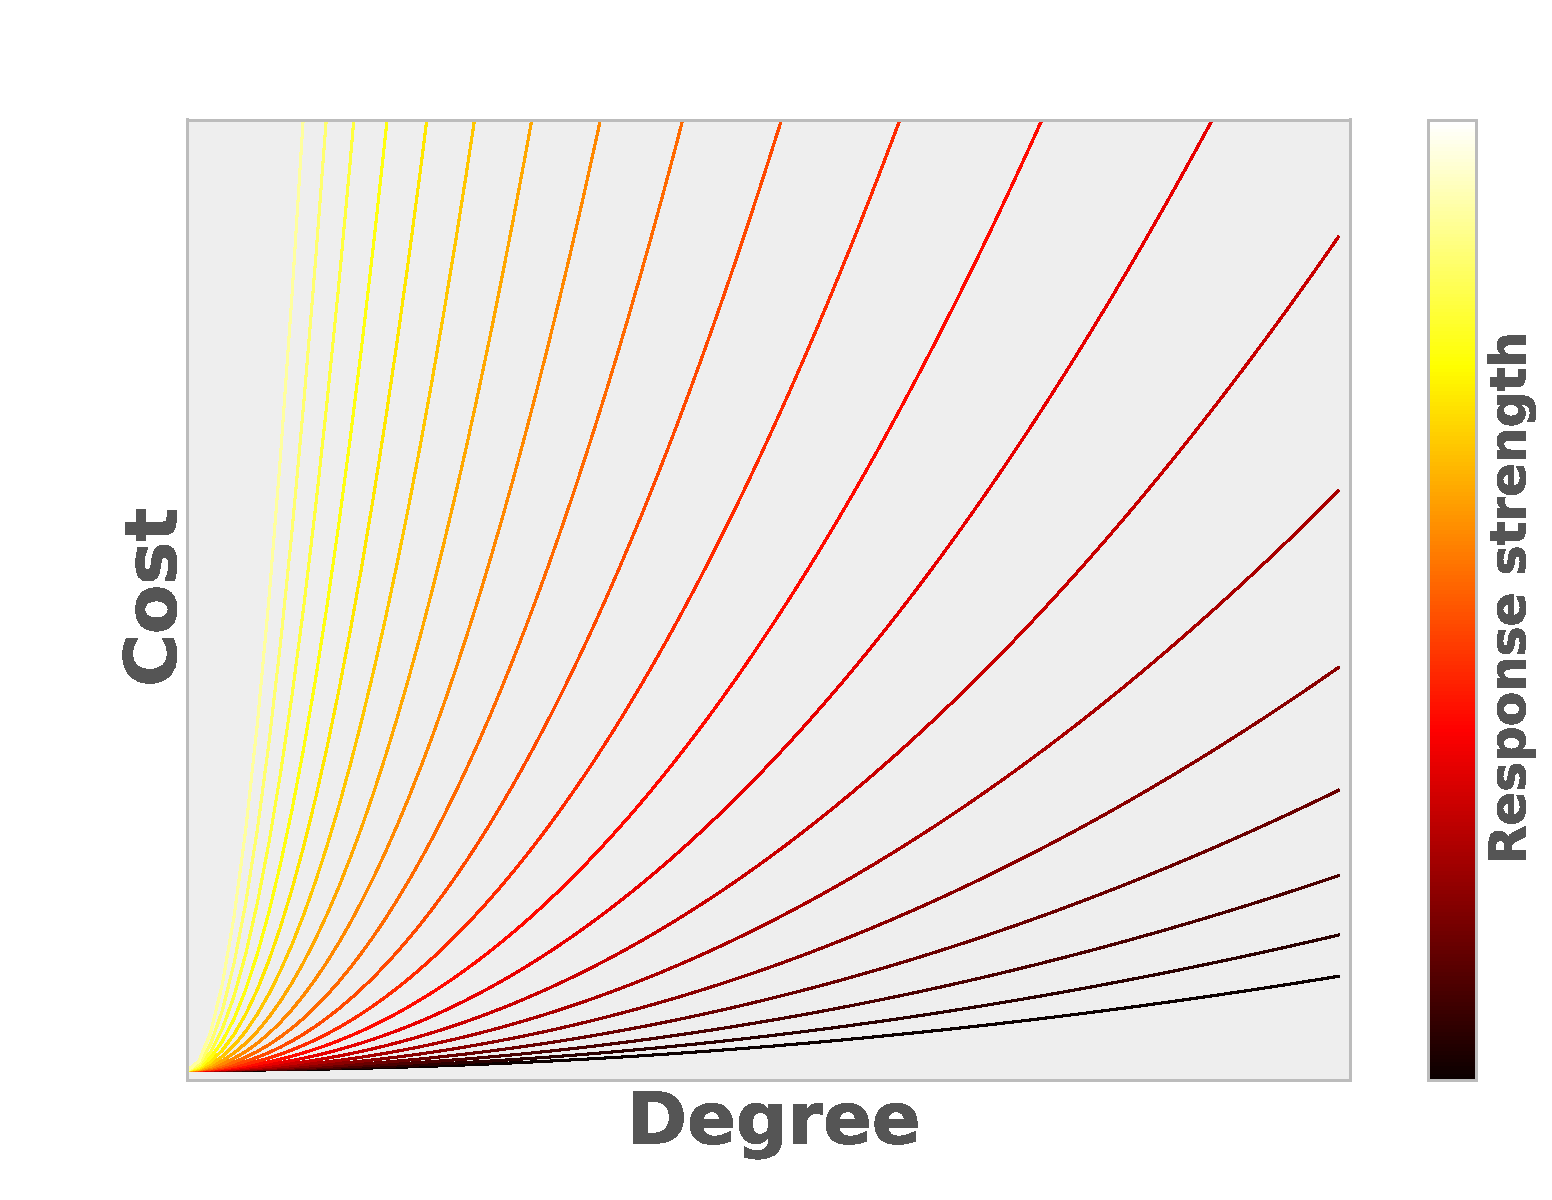
\includegraphics[width=0.8\textwidth]{cost_function.pdf}
\end{center}
\caption[Topological constraint in reverse-engineering]{
{\bf Schematic cost functions in relation to the connectivity and dynamic 
response of a gene.}
Possible cost functions that implement the topological constraint are
represented by parabolas with different curvatures. For instance, the 
cost function of strongly responding genes (bright color) increases
rapidly with the degree, such that genes with only a small amount of
connections are penalized and thus are forced to be sparsely connected.
By contrast, the cost function of moderately responding genes (dark color)
is rather flat. Therefore, these genes do not have any degree preference.
}
\label{fig:cost_function}
\end{figure}

Instead of the single-objective optimization, the multi-objective
optimization tries to find a set of solutions that are mutually non-dominating~%
\citep{Deb2002,Higuera2012}.
That is, by moving from one solution to another in this optimal solution set,
one may gain performance according to one objective, but always has to 
sacrifice the other objectives.
Previous attempts have been made to incorporate the topological information
into the multi-objective optimization framework~\citep{Spieth2005}. However,
it is mainly an implementation of the sparsity assumption, and does not
distinguish between genes with different response strengths. The lesson
learned in the current study may provide much richer information to the 
multi-objective optimization algorithm.

A second option to impose the topological constraint is the Bayesian network
approach. A Bayesian network is a probabilistic graphical model that represents 
a set of random variables and their conditional dependencies via a directed 
acyclic graph (DAG). The inference of the Bayesian network structure can be 
expressed as the maximization of the conditional posterior probability of 
the network structure given the data $\mathrm{Pr}(G|D)$, according to Bayes' rule,
\begin{equation}
\mathrm{Pr}(G|D) \propto \mathrm{Pr}(D|G) \cdot \mathrm{Pr}(G)
\end{equation}
where $\mathrm{Pr}(D|G)$ is the marginal likelihood of the data given a network 
structure and $\mathrm{Pr}(G)$ is then the prior probability of the network 
topology. Instead of using a uniform topological prior, one can specify 
different probability distributions for nodes with different responses~%
\citep{Friedman1998,Huang2007}.

As examples, \cite{Pe'er2002} introduced a method that examines only
those networks in which a small number of
regulators explain the expression of all other
genes. The restriction to such a
network architecture forces the learning procedure to identify the most pronounced regulators in the data set. It also simplifies the
learning procedure, which leads to statistical
and computational advantages. The work by \cite{Boeck2012} is based on the idea 
that biological 
networks are usually centered around a few hubs. More specifically, they modelled gene regulation using a Bayesian network with discrete, Boolean nodes. A hierarchical prior is employed to identify hub genes. The first layer of the prior is used to regularize weights on edges emanating from one specific node. A second prior on hyperparameters, in turn, controls the magnitude of the former regularization for different nodes. The net effect is that central nodes tend to form in reconstructed networks.

\section{Transcriptome-proteome correlation and time-scale 
separation}
Throughout \ref{chap:flow}, we have been advocating the 
separation of the transcript and protein activity. As a first
result, the phenotypical difference of the H838 cells between
the heterogeneous and the homogeneous coculture cannot be
translated back to the transcriptome response. In other words,
the H838 transcriptome is hardly differentially regulated
between the heterogeneous and the homogeneous coculture. 
Such a weak transcriptome response can be due to the priming
of the tumor cells with the endothelial cells before the
scratch/measurement begins. Within the 3 days coculture
before the confluency, tumor cells and endothelial cells
may have already exchanged signalling molecules and adapted
to each other's needs. Therefore, during the measurement
period, the transcriptome response in H838 cells 
under both heterogeneous and homogeneous conditions
may have gone back to the similar baseline.

The phenotype, however, is detectable both experimentally
and by inference from the basal gene set enrichment analysis.
This underlines again the divergence of the transcriptional
program in the tumor cells over time in the heterogeneous
and homogeneous cocultures. At the time of the phenotype
change, the transcriptional regulation is largely finished
and it is the proteins that are actually executing and
developing the phenotype. We acknowledge that the general 
protein
activity cannot be deduced from the transcriptome response.
However, the activity of the DNA-binding transcription
factors, which regulate the transcriptome, can be
inferred from the activity of their target genes.
More specifically, when considering all target genes of
a certain transcription factor as a group, one can ask
the question, whether this transcription factor target
group is significantly up-regulated compared to the
background group. The assumption we make here is that the actual
activity of a transcription factor correlates with 
the expression of its target genes, which is fairly
plausible.

The study of \cite{Jothi2009} highlights the discrepancy
between the transcript and protein level regulation of
transcription factors. The authors first classified a
yeast transcriptional network into a hierarchical
structure by a vertex sort algorithm. It was found that
transcription factors in different layers of the
hierarchical framework have distinct dynamic properties.
For instance, the top-layer transcription factors are
less abundantly expressed than the middle and bottom
layer. However, the protein products of the top-layer
transcription factors have a much richer amount than
the rest. This seemingly counter-intuitive fact can be explained by
the low degradation rate of the top transcription
factor proteins. Therefore, instead of the mRNA 
expression alone, it is rather the interplay between
the translation efficiency, degradation and 
post-translational modification that determine the
protein activity of a certain gene.

In order to decipher the signal flow in the cellular
interaction network and to identify the key 
transcriptional regulators, it is thus not sufficient
to only look at the transcriptome response of the
transcription factors. It is notable that transcription
factors are in general lowly expressed%
~\citep{Vaquerizas2009}, and they have decoupled
dynamic properties between the protein and transcript
level. 
In our example of the tumor-stroma interaction study, 
we proposed a time-scale separated,
integrative ansatz to first infer active 
transcription factors from the gene set enrichment 
analysis and then predict the most likely
signal path in the protein interaction network by 
random walk.

\section{Network inference by transcription factor binding site prediction}
We have seen in \ref{chap:flow} that transcription factors act as a key player
in relaying the information from the protein interaction network to the
transcriptional machinery, and thus bridging these two cellular processes
of different time scales. As a result, the understanding of how transcription
factors trigger the downstream gene regulation or how they bind to target genes
is of great importance. For instance, in the integrative signal flow approach
presented in \ref{chap:flow}, we inferred the putatively active transcription
factors by a target gene set enrichment analysis. The accuracy of the prediction
can be naturally improved if we have better knowledge about
the binding between transcription factors and the 
promoter region of their target genes. 
Although experimental techniques,
such as chromatin immunoprecipitation with microarray (ChIP-chip) or 
next-generation sequencing (ChIP-seq), are becoming mainstream in the study
of protein-DNA interactions, such data are still relatively scarce and 
computational methods to predict transcription factor binding sites (TFBS) are
greatly needed. 

Prediction algorithms come in two flavors~\citep{Das2007}: 
(1) based on the
assumption that co-expression implies co-regulation, genes are 
first clustered according to their expression values, the promoter sequences
of co-expressed genes are then searched for the over-representation of 
binding motifs; (2) alignment is performed for orthologous promoter sequences of a single gene from multiple species, the conserved sequence indicates a putative
binding motif according to phylogenetic footprinting. Depending on the 
technique used, motif detection algorithms can also be classified into
word-based (string-based) methods that mostly rely on exhaustive enumeration, i.e., counting and comparing oligonucleotide frequencies, and probabilistic sequence models which
represent each binding motif by a position weight matrix (PWM) that characterize
the occurence of individual bases.
Among the PWM-based approaches, MATCH~\citep{Kel2003} is a popular choice, which 
defines the matrix/core similarity score between a position weight matrix and
a DNA sequence, regions with both scores above a customized cut-off are considered
as possible binding sites.

Despite the long-lasting research effort in transcription factor binding site
prediction and a large number of proposed algorithms, the prediction accuracy 
is still sub-optimal and the false positive rate rather high. The limitation of
prediction algorithms has also been studied in an information theoretical
framework~\citep{Wunderlich2009}, where the miminal information required to identify a motif $I_{min}$ can be calculated from the size of genome ($N$) as
\begin{equation}
I_{min}=\log_2 N
\end{equation}
This minimal information can then be compared with the actual information ($I$) 
contained in individual position weight matrices (PWM).
\begin{equation}
\displaystyle I = -\sum_{i,j}p_{i,j} \cdot \log(p_{i,j})
\end{equation}
where $p_{i,j}$ is the frequency of base $i$ at the position $j$. \ref{fig:pwm_ic}
illustrates the information content of different species-specific position 
weight matrices from the TRANSFAC database~\citep{Matys2003b} (Release 2012.3). 
It is obvious that
the majority of the vertebrate PWMs has an information content below the 
minimal required information for fruit fly and human. This discrepancy is most
pronounced for the human genome, which pinpoints the difficulty of detecting 
transcription factor binding motifs from the human DNA sequence.

\begin{figure}[!ht]
\begin{center}
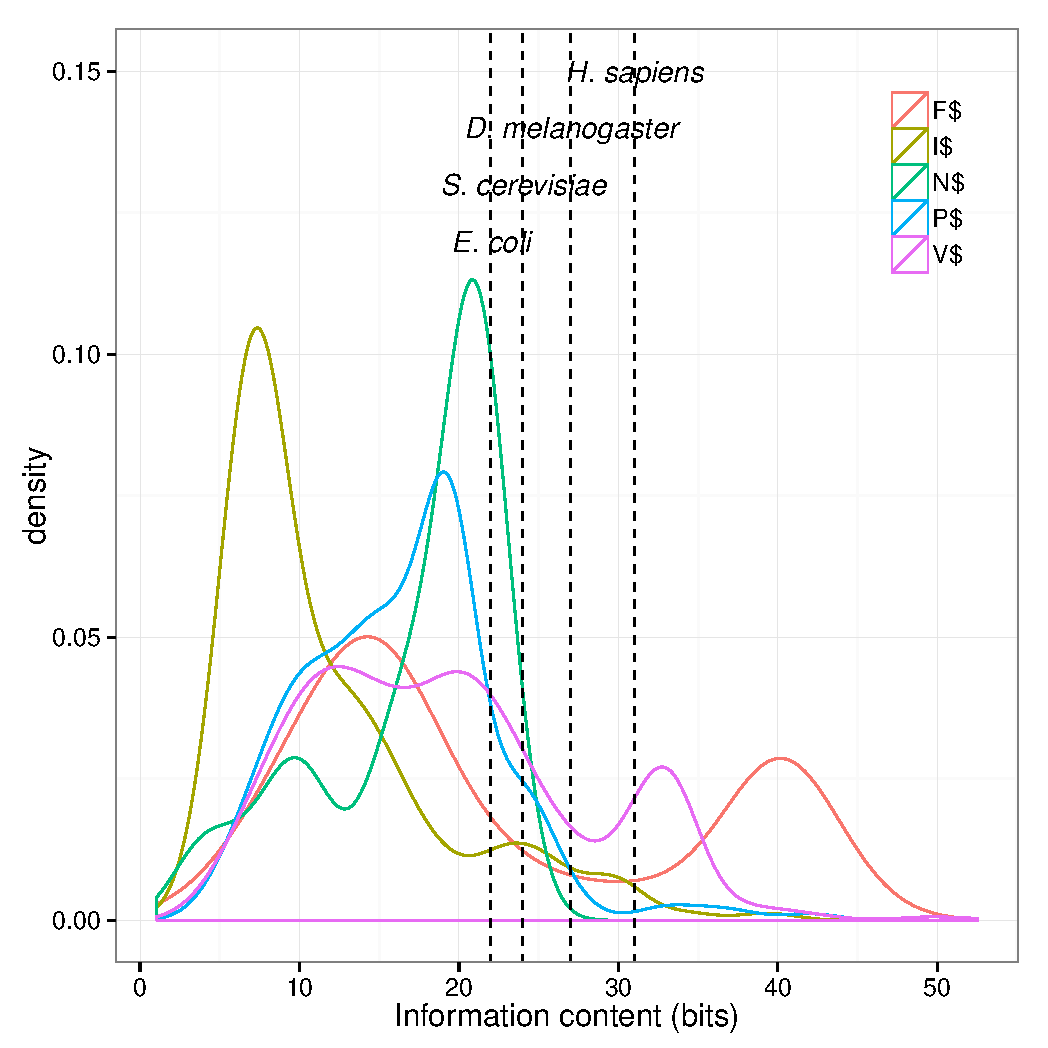
\includegraphics[width=0.8\textwidth]{pwm_ic.pdf}
\end{center}
\caption[Information content of position weight matrices]{
{\bf Distribution of the information content for position weight matrices in 
the TRANSFAC database.}
Shown are the distributions of information content in bits for species-specific
position weight matrices (PWM) in the TRANSFAC database. (Fungi: F\$, Insect: I\$,
Nematode: N\$, Plant: P\$ and Vertebrate: V\$) Vertical dashed lines denote
the calculated minimal information required to be able to identify a motif from
the genomic sequence using a particular PWM. (From left to right: \emph{E. coli, 
S. cerevisiae, D. melanogaster, H. sapiens})
}
\label{fig:pwm_ic}
\end{figure}

Yet other lines of evidence pointing to the difficulty of TFBS prediction are
discussed in \cite{Babu2004}. For example, 2604 human proteins are predicted to
have a DNA-binding domain, however, there are currently only 228 and 281 
transcription
factor binding motifs annotated in JASPAR~\citep{Sandelin2004} and TRANSFAC 
respectively. We can speculate that either we only know 10\% of the transcription
factors or the other DNA-binding proteins are not functional in the transcription
process. In either case, a better knowledge about the unknown DNA-binding
proteins is necessary to understand the transcriptional regulatory network.
In comparison to prokaryotes, the eukaryote transcription factor binding motifs 
are usually shorter, thus making the degeneracy of binding motifs more remarkable.
Therefore, one way to obtain more specificity might be achieved by the 
combinatorial regulation of transcription factors.
